% \textcolor{orange}{Section overview here.}

% \subsection{Architecture models}


% CPU architectures generally follow either the Von Neumann or Harvard model.
% The Von Neumann architecture uses a single memory space for both instructions and data, simplifying design but potentially causing bottlenecks due to shared bandwidth.
% In contrast, the Harvard architecture separates instruction and data memory, allowing simultaneous access and often better performance in embedded systems.
% As illustrated in Figure~\ref{fig:archimodels}, in a Harvard architecture, instructions and data might be isolated in different physical buses, while they must share physical resources in a Von Neumann architecture.

% \subsection{Basic CPU design}

% Modern CPU design incorporates several architectural features aimed at improving performance and efficiency.
% One fundamental concept is pipelining, which allows multiple instruction stages (fetch, decode, execute, etc.) to be processed simultaneously across different parts of the CPU, increasing throughput.
% To handle the uncertainties in instruction flow, branch prediction is employed.
% It anticipates the direction of conditional branches to minimize stalls.
% However, incorrect predictions can lead to the execution of instructions along the wrong path, a phenomenon managed by transient (or speculative) execution.
% This mechanism allows the CPU to proceed with predicted paths while preserving the ability to discard erroneous computations if the prediction was incorrect.
% Although effective, transient execution has introduced new classes of security vulnerabilities where the observable behavior of the CPU, such as its timing or the sequence of accessed memory addresses, can leak sensitive information to software concurrently running on the CPU~\cite{kocher2019spectre, lipp2018meltdown, armsecure,bhattacharyya2019smotherspectre,van2018foreshadow,canella2019fallout,horn2018speculative,maisuradze2018ret2spec,schwarz2019zombieload,schwarz2019netspectre,stecklina2018lazyfp,van2019ridl,ragab2021crosstalk,van2020lvi,van2021cacheout, ragab2021rage}.

In this section, we provide background on SoC platforms, timing side-channels and non-interference properties.

\subsection{SoC platforms}

\begin{figure}[t]
    \begin{center}
    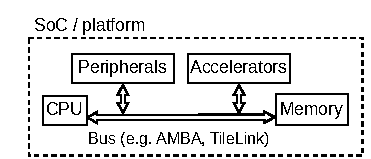
\includegraphics[width=0.8\columnwidth]{figures/exampleplatform/exampleplatform.pdf}
    \end{center}
    \vspace*{-1em}
    \caption{\label{fig:exampleplatform}
        Example SoC platform architecture.
    }
    \vspace*{-1em}
\end{figure}

In this paper, we use the words SoC and platform interchangeably to refer to the integrated circuit that incorporates all components of a computer onto a single chip.
As illustrated in Figure~\ref{fig:exampleplatform}, SoC platforms may integrate various components, including CPUs, memory, and peripherals, to provide a complete computing solution.
The communication between these components is typically managed through standardized bus protocols, such as AMBA~\cite{arm_amba} and TileLink~\cite{tilelink_spec}.
Note that the bounds of components are not always clear-cut.
For example, caches can be considered part of the CPU or of the platform.

\subsection{Timing side-channels}

Multiple hardware optimizations, such as caches and branch predictors, learn and exploit patterns in program execution to improve performance.
In particular, the execution time of later instructions may depend on the outcome of earlier instructions.
For example, accessing a cache line might be faster if the line has been brought into the cache recently by a prior memory access to a nearby location.
Timing side channels can result from such optimizations when the timing of a program's execution depends on secret data.
Constant-time programming techniques, such as not using secret data as array indices, aim to ensure that secrets do not influence the execution time of a program through such channels~\cite{OsvikShamirTromer2006CacheAES,AlmeidaEtAl2016CTVerif}.

\subsection{Information Flow Tracking}
\label{subsec:ift}

\begin{figure}[t]
    \begin{center}
    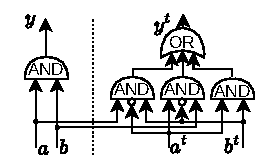
\includegraphics[width=0.5\columnwidth]{figures/glift/glift.pdf}
    \end{center}
    \vspace*{-1em}
    \caption{\label{fig:glift} Taint tracking at gate level~\cite{tiwari2009complete}. Left: original circuit. Right: Added instrumentation for taint tracking. The original inputs are $a$ and $b$. The taint bits corresponding to $a$ and $b$ are respectively $a^t$ and $b^t$. The output taint bit $y^t$ indicates whether the output is tainted, i.e., influenced by the tainted inputs.}
    \vspace*{-1em}
\end{figure}

\begin{figure}[t]
    \begin{center}
    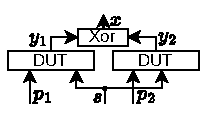
\includegraphics[width=0.5\columnwidth]{figures/miter/miter.pdf}
    \end{center}
    \vspace*{-1em}
    \caption{\label{fig:miter} Miter circuit. The two instances of the same design under test are supplied with the same secret data $s$ and unconstrained $p_1$ and $p_2$ public data. The output bit $y$ (i.e., instantiated for the instances in the miter as $y_1$ and $y_2$) reveals secret data if $x=1$ is satisfiable.}
    \vspace*{-1em}
\end{figure}

Information flows capture properties such as confidentiality and integrity~\cite{hu2021hardware}.
First, they can be measured by augmenting the hardware design under verification with a synthesizable instrumentation that computes the propagation of taint bits~\cite{tiwari2009complete,ardeshiricham2017register,solt2022cellift,solt2024hybridift,ceesay2024mucfi} as shown in Figure~\ref{fig:glift}.
Second, they can also be compared using a so-called miter circuit, comparing the outputs of two copies of the design under test, where all the inputs except the sources are unconstrained, while all the others are equal as illustrated in Figure~\ref{fig:miter}.



\subsection{Hardware-software contracts}
\label{subsec:hw-sw-contracts}

% {\color{cyan}{

\para{Contract definition}
Hardware-software contracts~\cite{guarnieri2021hardware} split confidentiality responsibilities between the CPU and the software that it executes.
For a given program, an initial microarchitectural state, and the contents of memory, the contract fixes an execution mode and an observation mode.
The \emph{execution mode} determines which instructions (beyond those architecturally present) may be executed and generate events.
The \emph{observation mode} determines which of those events are exposed to an observer (possibly transiently), such as the addresses or values involved in memory accesses. Under these two choices, the CPU's behavior is summarized as a sequence of observable events known as a hardware trace~\cite{guarnieri2021hardware,oleksenko2022revizor}.

% \subsection{Hardware-software contract verification}
% \label{subsec:hw-sw-contracts-verification}

% {\color{cyan}{

\para{Contract verification}
Multiple independent verification efforts have been conducted to ensure that hardware-software contracts are upheld during program execution, in particular regarding constant-time behavior~\cite{dinesh2024conjunct,ceesay2024mucfi,guarnieri2021hardware,tan2025contractshadowlogic,dinesh2025h,hsiao2024rtl2mmupath,wang2023specification}.
Most techniques consider a fixed contract~\cite{dinesh2024conjunct,ceesay2024mucfi,tan2025contractshadowlogic,dinesh2025h}.
Others leverage custom, non-trivial insights and techniques to verify specific contracts~\cite{hsiao2024rtl2mmupath,wang2023specification}.

\para{Discussion}
In this paper, we will introduce \pics, a novel abstraction for reasoning about platform-induced timing side-channels, and hence about different hardware-software contracts.
We will introduce a synthesizable instrumentation generic across verification techniques.

% To understand information propagation and split responsibilities between hardware and software, past work has formalized the sequence of observable events produced by a CPU when executing a given program as a function of the initial microarchitectural state, the program and the data in memory.
% This observation sequence is referred to as a hardware trace~\cite{oleksenko2022revizor}.
% Possible hardware traces are specified as a contract~\cite{guarnieri2021hardware}, which stipulates an execution mode and an observation mode.
% The \emph{execution mode} determines which instructions will be executed and cause observable events, in addition to the instructions architecturally present in the executed program.
% The \emph{observation mode} determines the events that are exposed to the observer by (potentially transiently) executed instructions when executing the program, for example, disclosing addresses or values that correspond to memory accesses.
% }


% \fls{Maybe add some more detail}
% \fls{R3. There is a significant amount of jargon related to security and side-channel attacks that is likely not familiar to the average ICCAD attendee, and is not really adequately introduced or explained.}

% \begin{equation}
% \vspace*{-.3em}
% \label{eq:isatrace}
% % \text{ISA}(P, M_p, M_s) = \text{ISA}(P, M_p, M'_s)
% \text{ISA}(P, M_s) = \text{ISA}(P, M'_s)
% \end{equation}
% \begin{equation}
% \label{eq:microtrace}
% % \text{Micro}(P, M_p, M_s) = \text{Micro}(P, M_p, M'_s)
% \text{Micro}(P, M_s) = \text{Micro}(P, M'_s)
% \end{equation}

% \para{Discussion}
% Verifying non-interference properties raises challenges not only in terms of properly mapping the property to the design under verification, but also in terms of completeness and performance.
% Existing work has proposed various approaches to address these challenges, including decisions on the observation mode and specific assumptions that accelerate the verification process.
% }


% In the rest of this paper, we consider $M_p$ as part of the program $P$.
% Intuitively, non-interference properties express that an observer cannot infer more information about the input of a program execution on a given CPU than what is allowed in a given contract.


% \subsection{Non-interference Properties}
% \label{subsec:non-interference}

% Past work has formalized the sequence of observable events produced by a CPU as a function of the sequence of instructions and data that it processes, starting in a given microrachitectural state.
% This sequence is referred to as a hardware trace~\cite{oleksenko2022revizor}.
% A hardware trace is a function of a contract~\cite{guarnieri2021hardware}, which stipulates an execution mode and a set of observer modes.
% The execution mode determines which instructions will be executed speculatively in addition to the architecturally executed instructions.
% The observer mode determines the events that are exposed to the observer, for example, disclosing addresses or values of memory accesses.

% Non-interference properties express that the observable behavior of a CPU is independent of the secret data processed by the CPU, and hence these properties add the notion of a secret information to the contract. 
% Formally, a CPU implementation satisfies non-interference if for all programs $P$, and all public memory valuations $M_p$ and pairs of secret valuations $M_s$ and $M'_s$, Equation~\ref{eq:isatrace} implies Equation~\ref{eq:microtrace}, i.e., if the ISA observations for the triples $(P, M_p, M_s)$ and $(P, M_p, M'_s)$ are the same, then the microarchitecture's observations for the triples $(P, M_p, M_s)$ and $(P, M_p, M'_s)$ are also the same.

% % Intuitively, non-interference properties express that an observer cannot infer more information about the input of a program execution on a given CPU than what is allowed in a given contract.

% \begin{equation}
% \vspace*{-.3em}
% \label{eq:isatrace}
% \text{ISA}(P, M_p, M_s) = \text{ISA}(P, M_p, M'_s)
% \end{equation}
% \begin{equation}
% \label{eq:microtrace}
% \text{Micro}(P, M_p, M_s) = \text{Micro}(P, M_p, M'_s)
% \end{equation}


% Previous work has proposed verifying several property classes varying in terms of the observation mode, e.g., whether we expect the address of load and store instructions to be observable or not~\cite{guarnieri2021hardware}.
% Follow-up work unanimously verifies contracts with an observation mode that focuses on instruction commitment timing, i.e., verify whether secret information can influence the timing of some instruction commitment~\cite{tan2025contractshadowlogic,ceesay2024mucfi,dinesh2024conjunct,dinesh2025h}.
% Regarding the execution mode, apart from \ucfi~\cite{ceesay2024mucfi} arguably relies on the sequential execution mode, where instructions are executed one at a time, the existing work focuses on the always-mispredict execution mode, which implies that instructions might be executed speculatively.
% Note that these aspects are not always discussed in detail in the literature.


% % Several properties are instances of non-interference properties.
% % The Safe Instruction Set (SIS) property restricts the programs $P$ to programs made exclusively of a given set of instructions defined as safe.
% % The Speculative Non-Interference (SNI) property does not impose a restriction on the instructions architecturally composing a program.
% % Both properties take the always-mispredict (\emph{spec}) execution mode, which implies that all instructions are executed speculatively.


% \textcolor{red}{TODO Establish the link between equality constraints and taints}

% % Hardware designs are generally described at the Register Transfer Level (RTL) in languages such as Verilog.
% % RTL is an abstraction level describing the behavior of digital circuits in terms of binary data flows between registers, and the arithmetic or logical operations that are performed on the data.
% % Modules describe the hierarchy of a design~\cite{verilog}.
% % All digital circuits can be described down to a (large) netlist of logic gates, such as AND, OR, and simple stateful elements such as flip-flops and latches.
% % Electronic Design Automation (EDA) software often first transforms the RTL description into a netlist of macro-cells, which is the preferred intermediate representation for optimizations, transformations and synthesis~\cite{wolf2013yosys}.

% % \subsection{Hardware DIFT}

% % An information flow (also known as taint flow) between a source and a sink signifies that changes in the valuation of the source signal can affect the valuation of the sink signal.
% % Computing whether a signal A should be tainted is equivalent to iterating through all valuations of all tainted signals, and observing whether A is affected.
% % % This tainting is done out-of-band, e.g., by using a parallel taint bit for each bit in the design~\cite{tiwari2009complete}.
% % % Hardware Dynamic Information Flow Tracking (DIFT) is a technique that tracks the flow of information through a digital design.
% % Information Flow Tracking (IFT) can be used to detect information leaks like side-channel attacks or to detect bugs in a design~\cite{tiwari2009complete,solt2022cellift,ardeshiricham2017clepsydra,oberg2011information,oberg2014leveraging}.
% % Dynamic IFT (DIFT) instruments designs by concretely inserting additional logic to track the flow of information through the original design, while the original design's functionality remains unaffected.
% % This instrumentation allows following information flows through the design at runtime, typically during simulation, or when proving formal properties.
% % Several abstraction levels have been proposed for DIFT instrumentations: gate level (GLIFT)~\cite{tiwari2009complete}, RTL (RTLIFT)~\cite{ardeshiricham2017register}, and most recently the Yosys macro-cell level (CellIFT)~\cite{solt2022cellift}.

% % % \textcolor{red}{TODO: Probably put the following in the intro section.}
% % The existing instrumentation mechanisms~\cite{tiwari2009complete,solt2022cellift} hit a scalability wall when instrumenting deep memories (i.e., memories with many words) such as the default caches of CVA6~\cite{zaruba2019cost}, Rocket~\cite{asanovic2016rocket}, BOOM~\cite{asanovic2015berkeley} and OpenC910~\cite{chen2020xuantie}.
% % Consequently, such designs are sometimes adapted specifically for instrumentation~\cite{solt2022cellift}.
% % Some open-source designs are not much parametrizable in terms of memory sizes~\cite{chen2020xuantie,zaruba2019cost}, making their instrumentation difficult in practice, by incurring either a heavy manual effort, or significant performance overheads.

% % \subsection{Memories}

% % % A hardware design is generally intended to target ASIC or FPGA implementations, and often both.
% % At design time, the exact memory implementation (mega-cell for ASICs, BRAM for FPGAs) is usually abstracted away and only the memory interface is described.
% % The memory is instantiated as a black-box module that emulates the functionality for simulation purposes.
% % In particular, apart from a clock signal, memories have a data input and output, an address input, and some enable signals.
% % SRAMs are particularly area- and power-efficient memories, at the cost of providing access to only one element at a time, as opposed to standard cells, which may provide access to multiple elements concurrently~\cite{teman2016power,meinerzhagen2010towards,meinerzhagen2011benchmarking,marazzi2022protrr}.
